% !TEX program = xelatex

\documentclass[12pt, a4paper]{article}

\usepackage{fontspec}
\setmainfont[Ligatures=TeX]{Linux Libertine O}

\usepackage[rgb]{xcolor}
\definecolor{lightblue}{rgb}{0.4, 0.6, 0.9}
\usepackage[hidelinks, colorlinks=true, linkcolor=lightblue, urlcolor=lightblue, citecolor=lightblue, filecolor=lightblue]{hyperref}

\usepackage{indentfirst}
\usepackage{graphicx}
\usepackage[left=1.5cm,right=1.5cm,top=1.5cm,bottom=1.5cm]{geometry}
\usepackage{lipsum}
\usepackage{caption}
\usepackage{subcaption}
\usepackage{dirtytalk}
\usepackage{cancel}
\usepackage{amsmath}

\usepackage{minted}


\usepackage{nameref}
\newcommand*{\fullref}[1]{\hyperref[{#1}]{\ref*{#1} \nameref*{#1}}} 

\setlength{\parskip}{0.8em}

\usepackage{epigraph}


\graphicspath{{assets/}}


\begin{document}



\title{
Neural network training workflow Ilastik\\[1cm]

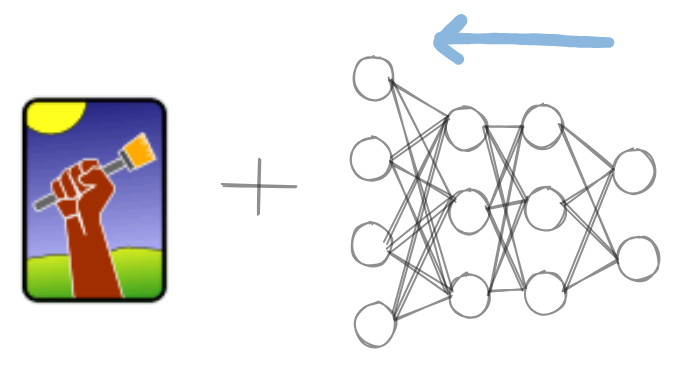
\includegraphics[width=0.5\textwidth]{ilastik-logo.png}
}

\author{Theodoros Katzalis}


\date{10/2024}

% \date{\today}

\sloppy
\maketitle

{
%\renewcommand*\contentsname{Περιεχόμενα}
\hypersetup{linkcolor=black}
\tableofcontents
}

\clearpage

\section{Introduction}

Ilastik is a desktop application that bridges the gap between machine learning and out of the box functionality intended for the bioimaging domain. For more about ilastik, check the documentation at \url{https://ilastik.github.io/}.

The main takeaway of the currently supported functionality is that training is only possible with shallow models (e.g. random forests), and neural network workflows are used only for inference. Our endeavor would be to integrate neural network training in ilastik.

The main motivation of this work originates by the shallow to deep project \cite{Matskevych2021.11.09.467925}. Its core idea is that domain adaptation can achieve greater performance by incorporating a shallow model as a preliminary step. Instead of trying to learn the mapping of raw data to the ground truth segmentations, we can learn the mapping of the output of the shallow model to the ground truth segmentations (enhancer). For a new dataset, the pretrained enhancer attempts to correct the result of the new trained shallow model. A subsequent part would be as well to train a new neural network model (segmentor) for semantic segmentation from raw images, but this time to use the output of the pretrained enhancer as pseudo labels. The whole workflow can be illustrated in the following figure:

\begin{figure}[h!]
    \centering
    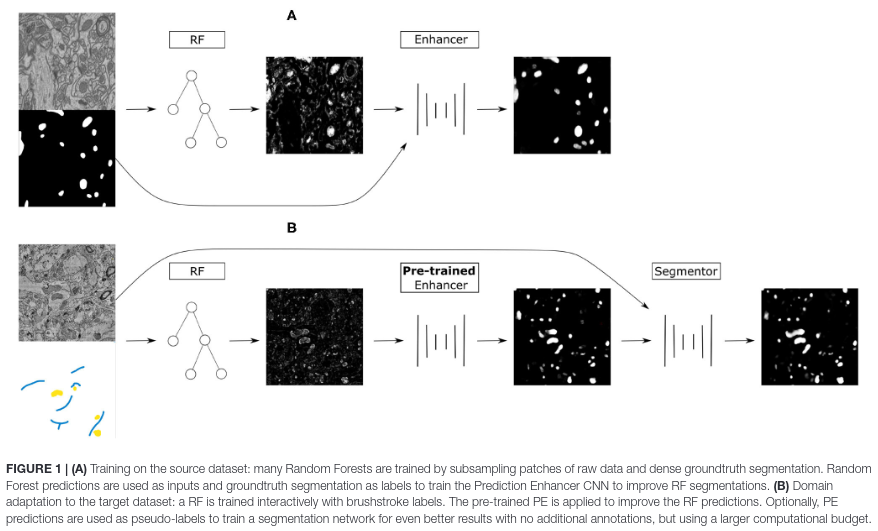
\includegraphics[width=0.8\textwidth]{shallow2deep.png}
    \caption{Shallow to deep \cite{Matskevych2021.11.09.467925}}
\end{figure}

Having as a reference point the above workflow, ilastik provides the functionality for training the random forests, but not the enhancer and the segmentor. Our goal is to achieve the whole workflow with ilastik.

Effectively to realize the above, we will attempt to implement a supervised machine learning workflow in ilastik. This will serve as the starting point for more sophisticated training workflows in the future. For next steps, refer to \fullref{sec:next_steps}.

\clearpage

\section{Ecosystem}

\begin{figure}[h!]
    \centering
    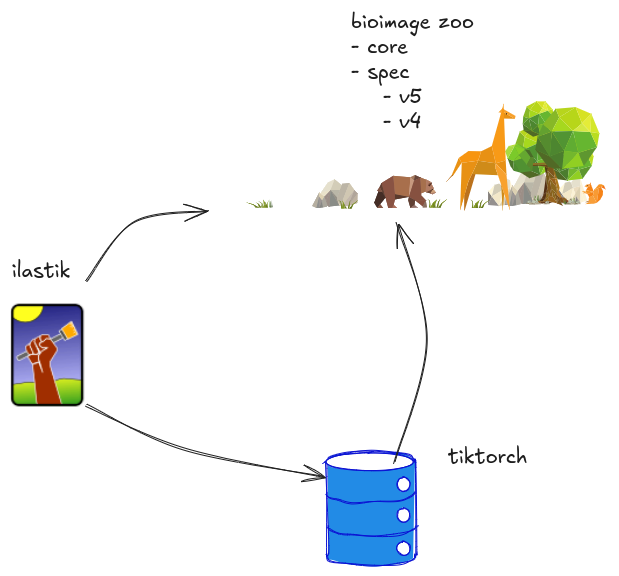
\includegraphics[width=0.8\textwidth]{ecosystem.png}
    \caption{Ecosystem}
\end{figure}


\section{Current state of tiktorch}

As we have seen tiktorch is our backend system to run the heavy load of neural networks. Let's see what is the current state of it.

producer-consumer

threads, processes, orchestration

\section{Lazyflow}

What kind of operators to use.

\section{Ilastik view}

How it would look like?


\section{Next steps}
\label{sec:next_steps}

One of the major bottlenecks with supervised machine learning and especially in the biological domain is the very expensive, and time-consuming process of data annotation.

\begin{itemize}
    \item Representation learning. Instead of trying to train from scratch a neural network in a supervised manner, would be very beneficial to make use of the latent space of representation learning methods.
    \item Integrate already trained models (e.g. bioimage zoo), allowing finetuning to them.
    \item Instance segmentation.

\end{itemize}

\clearpage

\bibliographystyle{plain}
\bibliography{bib.bib}



\end{document}